Following the steps outlined in Section~\ref{sec:method} results in a tKG comprising 1,513,398 quadruples across 365 timesteps, with 290,457 distinct nodes and 13 distinct relations. In this tKG, 1,424,956 quadruples originate from the ACLED dataset, 88,442 quadruples originate from the GTA dataset, containing information on in total 3,677 GTA interventions. In the following, we describe this tKG and provide insights from the conducted analysis.

\subsection{Temporal Knowledge Graph Analysis} 
We analyse the resulting tKG by computing and observing its graph properties over time. Figure~\ref{fig:graph_params_timeseries} illustrates these properties of the KG snapshots per timestep, including the number of triples (a), the number of nodes (b), the density (c), the mean node degree (d), and the maximum node degree (e). 
\begin{figure*}[!t]
\begin{minipage}{\textwidth}
	\centering
	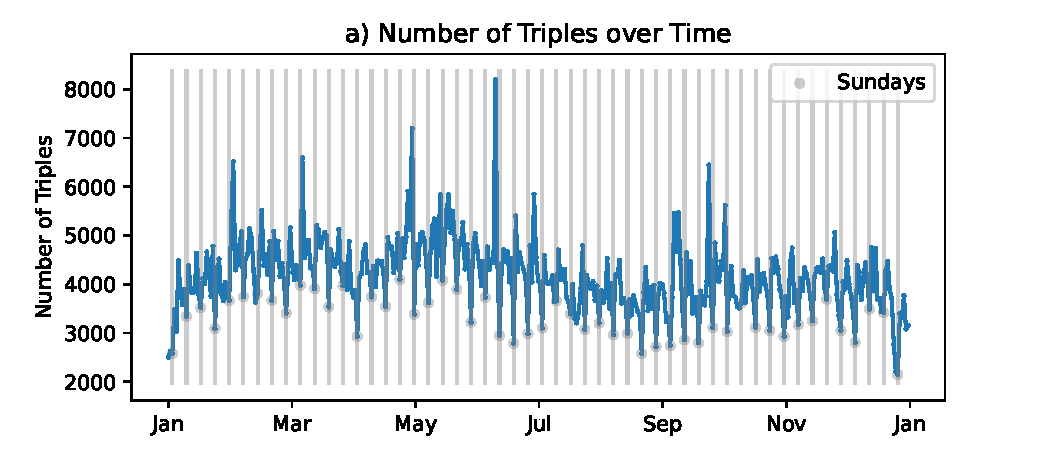
\includegraphics[width=0.49\textwidth]{figs/acled_subset_gta_aggregatedNumber of Triples.pdf}\\
\end{minipage}
\begin{minipage}{0.49\textwidth}
	\centering
	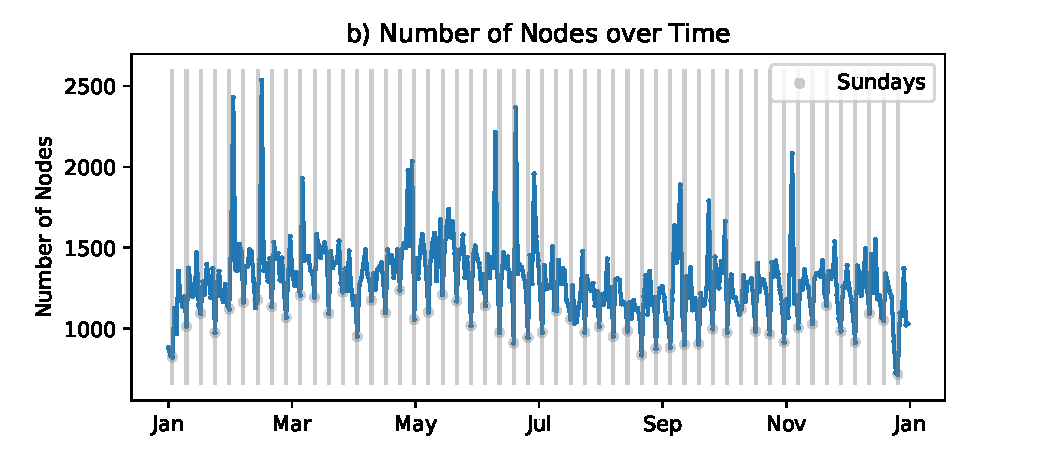
\includegraphics[width=\textwidth]{figs/acled_subset_gta_aggregatedNumber of Nodes.pdf}\\
\end{minipage}
\hfill
\begin{minipage}{0.49\textwidth}
	\centering
	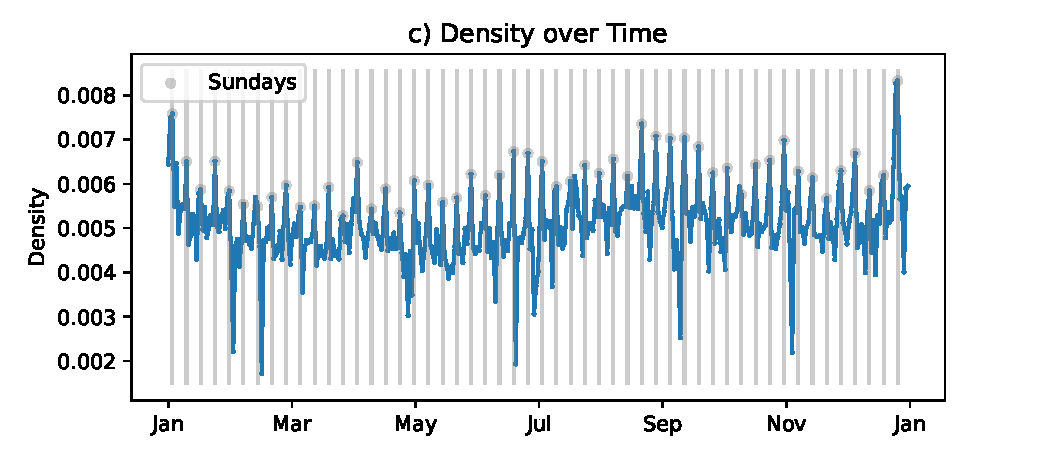
\includegraphics[width=\textwidth]{figs/acled_subset_gta_aggregatedDensity.pdf}\\
\end{minipage}
\begin{minipage}{0.49\textwidth}
	\centering
	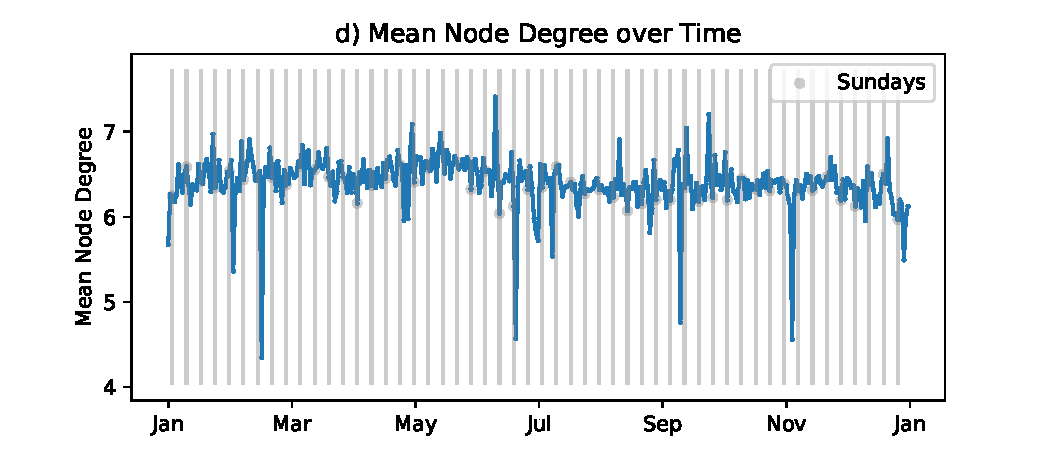
\includegraphics[width=\textwidth]{figs/acled_subset_gta_aggregatedMean Node Degree.pdf}\\
\end{minipage}
\hfill
\begin{minipage}{0.49\textwidth}
	\centering
	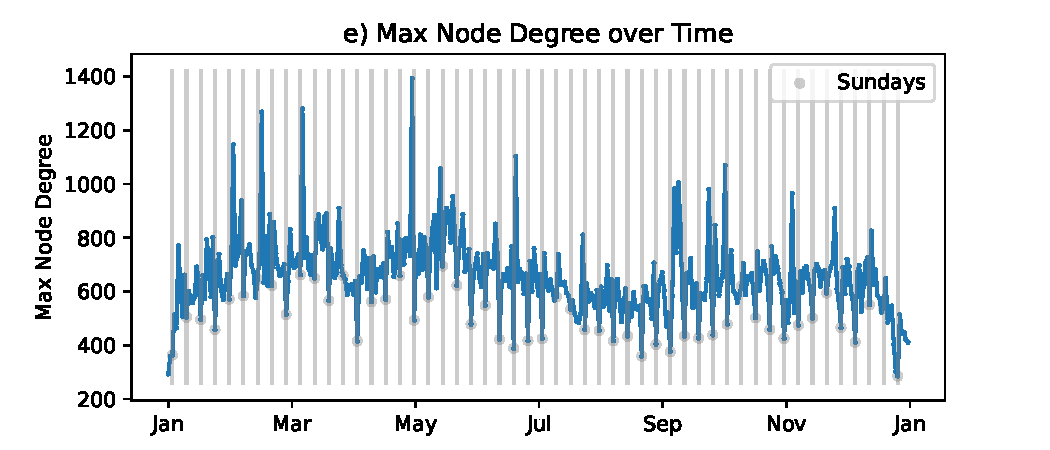
\includegraphics[width=\textwidth]{figs/acled_subset_gta_aggregatedMax Node Degree.pdf}\\
\end{minipage}
\caption{Graph properties over time, one entry per graph snapshot. All Figures show the year 2021. 
Grey lines and dots mark Sundays. (a) number of triples, (b) number of nodes, (c) density, (d) mean node degree, (e) max node degree.}  
\label{fig:graph_params_timeseries}
\end{figure*}

In the following, we describe some key observations: 
\begin{description}
    \item[Number of triples per timestep] With more than 2,500 triples in each timestep, this tKG is larger than the tKG datasets described in section \ref{sec:rel_work}.
    \item[Number of nodes per timestep] The tKG contains 290,457 unique nodes, but only a small subset of these nodes ($<1\%$) is present in each timestep, implying that many nodes do not appear frequently.
    \item[Density] The density varies between 0.002 and 0.007, indicating a relatively sparse graph\footnote{A fully connected graph has a density of 1.}.
    \item[Mean and Maximum Node degree] The maximum node degree is significantly higher ($>400\%$) than the mean node degree, indicating the existence of hub nodes with comparatively very high node degree.
    \item[Seasonality] The time series in (a) - (d) exhibit weekly seasonality. Sundays contain the lowest number of triples/nodes, the lowest node degree, and the highest density.
    \item[Outliers] Figure~\ref{fig:graph_params_timeseries} shows five peak days, containing a high number of nodes ($>2,100$), high number of triples ($>6,000$), low density ($<0.003$), low mean node degree ($<5$), and high maximum node degree ($>1000$). These days contain hub nodes that have more neighbors than hub nodes in other timesteps.
\end{description}

\subsection{Visualisation}
We show an exemplary tKG snapshot for the first timestep\footnote{To view the dynamic visualisation of the remaining timesteps, please run the script provided in our GitHub repository and adjust the dedicated slider.}
in Figure~\ref{fig:kg_static}. 
Nodes in orange are from GTA triples, blue nodes are from ACLED triples, and green nodes appear in both datasets.

The figure illustrates that the majority of triples are from the ACLED dataset. These blue triples contain a small number of hub nodes, linking to a significant amount of other nodes. These hub nodes consist of nodes representing event types such as \textit{Peaceful Protest}, nodes for prominent actors like \textit{State Forces} or numeric values like a node that denotes the number 1 (connected via the relation \textit{Number of Fatalities}). 
Further, the figure depicts orange hub nodes, i.e. hub nodes for the GTA dataset. This graph snapshot comprises 13 distinct GTA interventions across 7 GTA state acts. Each intervention has a varying amount of affected jurisdictions (ranging from 1 to 50) and has unique properties, such as affected products and sectors. The orange hub nodes are interventions with a large number of affected jurisdictions.
\begin{figure}
    \centering
    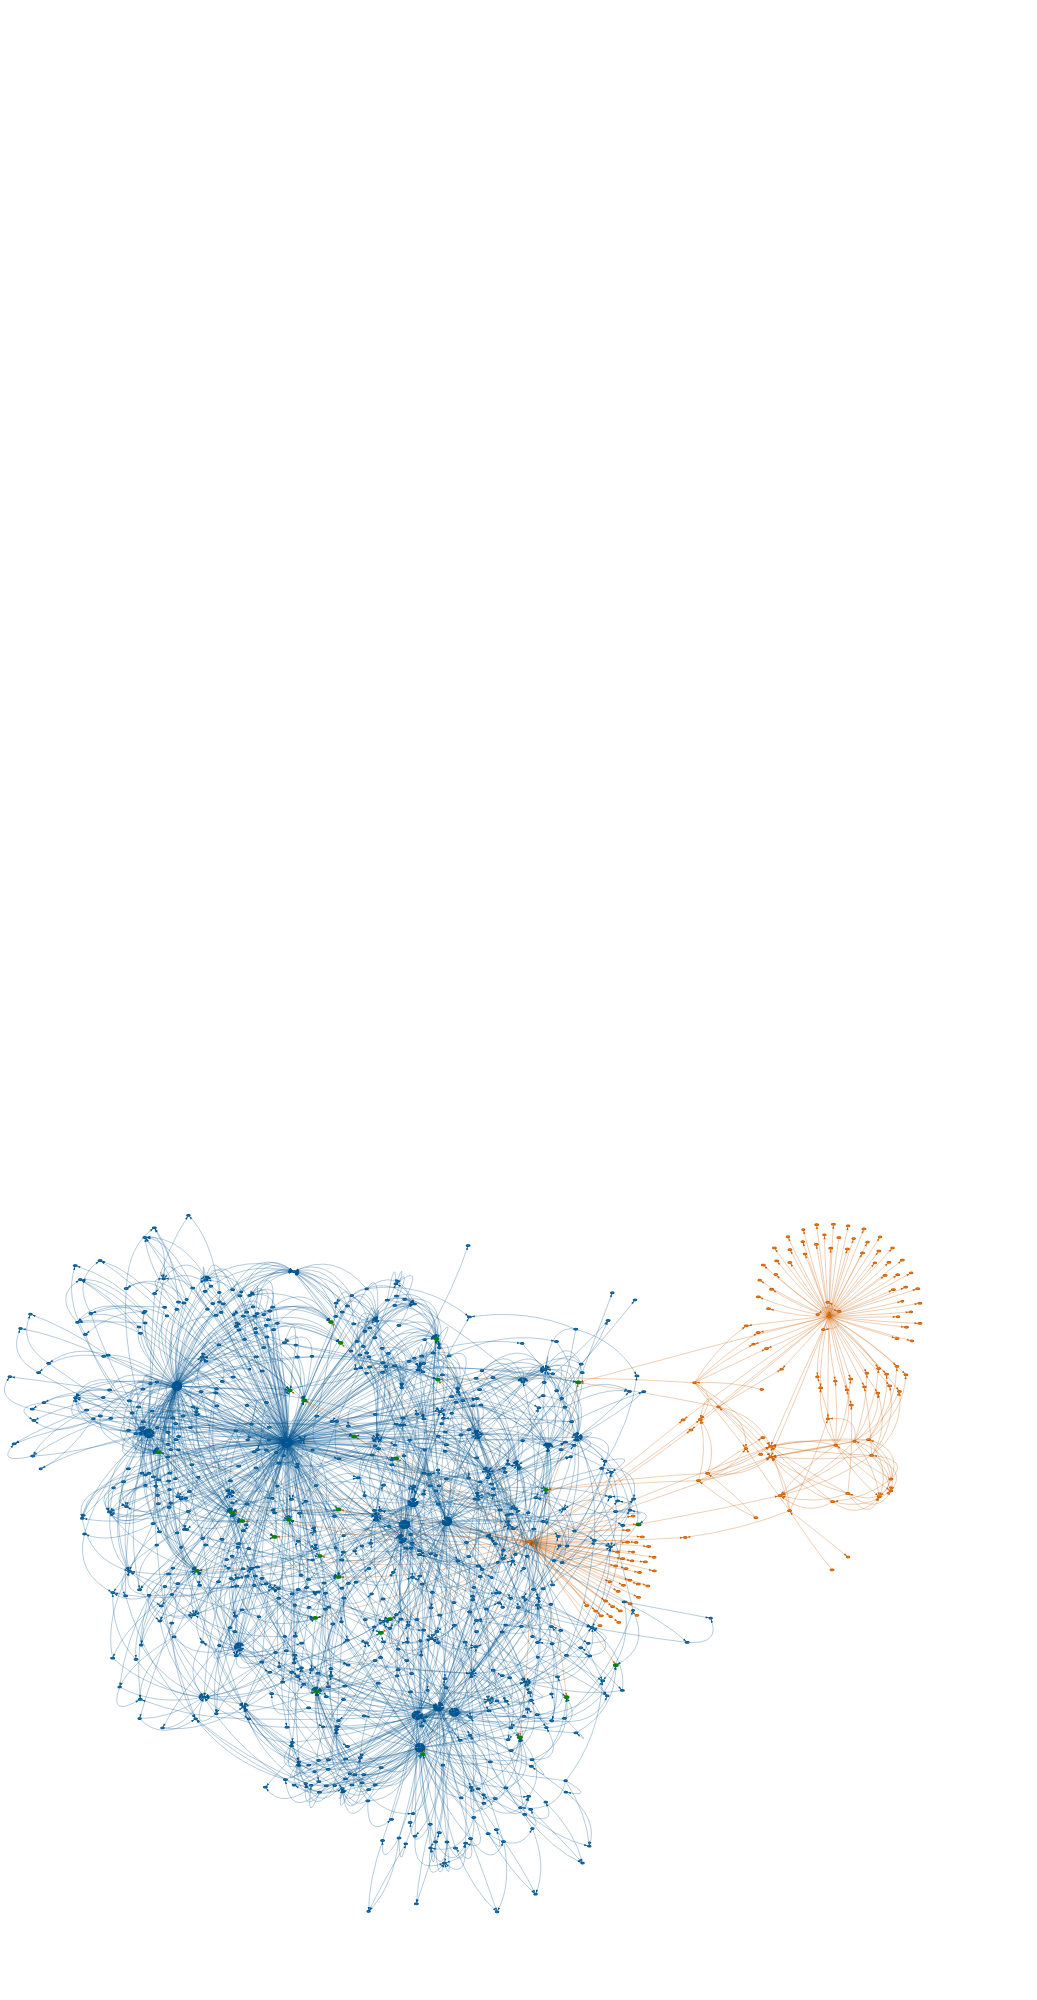
\includegraphics[clip, trim=0cm 3cm 0cm 42cm, width=1\textwidth]{figs/snap1_newcolors_horizon.png} %,trim=4.5cm 3cm 2.5cm 2cm,clip]
    \caption{Exemplary KG snapshot for the first timestep. Orange nodes are from GTA, blue nodes are from ACLED, and green nodes appear in both datasets. The majority of triples are from ACLED. Both, ACLED and GTA, contain a small number of hub nodes, linking to a significant amount of other nodes.}
    \label{fig:kg_static}
\end{figure}
\subsection{Challenges and Considerations for tKG Forecasting: Analysis Insights}\label{sec:takeaway}
The insights gained from the analysis help to define requirements for tKG Forecasting for the use case in Section~\ref{sec:intro}. 
Compared to the datasets in Section~\ref{sec:rel_work}, a tKG forecasting model for the given tKG dataset needs to handle a larger number of triples, and a significantly larger number of nodes. Moreover, the model must be capable of distinguishing hub nodes with a very high node degree from nodes with a low node degree, and of differentiating between these. 
Further, the model must be able to account for peak days and incorporate them into its predictions. An additional challenge is the capturing of seasonal information. For this reason, the forecasting model should have the capability to incorporate seasonal variations in its predictions.
